% Provenance (never printed): see sources/outline_sources.md (Year 3: the
% Rayleigh number; thermal boundary layers; slab pull and ridge push; plumes;
% post-glacial rebound and mantle viscosity). Brief: sources/book5/BRIEFS.md,
% ch. 6. Curves from figdata/bachelor-3/convection_scaling.py (PREM read only),
% gia_relaxation.py and ridge_push.py (on plate_cooling.py). Exercise and
% problem values in the Book 5 scratch calculator calc/ch06.py.
\chapter{Convección del manto y fuerzas motoras de las placas}\label{ch:b3:mantle-convection}

La costa del norte de Suecia emerge del mar a un ritmo de cerca de un centímetro al
año, diez mil años después de que el casquete de hielo que la cubría se fundiera.
Las orillas de la bahía de Hudson se elevan con la misma rapidez. Nada las empuja hacia arriba salvo el manto,
que fluye lentamente de vuelta bajo el lugar que el hielo había hundido. La velocidad
a la que el suelo recupera su posición pesa sobre la \omterm{def:b3:mantle-convection:gia}{viscosidad del manto}, y esa misma
viscosidad determina la rapidez con que el manto convecta y se mueven las placas. Este capítulo
se pregunta por qué el manto sólido convecta en absoluto, con qué rapidez debe fluir para transportar
el calor de la Tierra, qué fuerzas mueven las placas y qué dice el rebote del terreno
sobre la \omterm{def:b3:mantle-convection:gia}{viscosidad del manto}.
% ledger: vestol19:umea, zhao12:fenno, sella07:gia

\begin{recall}
La viscosidad, el flujo reptante de un fluido viscoso (las ecuaciones de Stokes
$\nabla p = \eta\nabla^2\mathbf u$, $\nabla\cdot\mathbf u = 0$), la ley de Stokes
para una esfera, el número de Reynolds y la flotabilidad están en los volúmenes
universitarios de los libros de física. La convección del manto y el rebote isostático se vieron en el
volumen de secundaria (año 12); el empuje de la dorsal y el tirón de la losa, en su parte de año 11.
La capa límite térmica, la litosfera térmica y la adiabática del manto se encuentran
en el volumen de primer año, en su capítulo sobre el balance térmico de la Tierra; los puntos calientes,
las plumas del manto y las grandes provincias ígneas en su capítulo sobre puntos calientes.
El \omterm{def:b3:lithosphere-thermal-models:half-space}{modelo de enfriamiento de semiespacio} figura en el \cref{ch:b3:lithosphere-thermal-models},
la flexión de la litosfera en el \cref{ch:b3:gravity-geodesy}, la \omterm{def:b3:seismology-imaging:tomography}{tomografía sísmica}
en el \cref{ch:b3:seismology-imaging}.
\end{recall}

\section{Por qué convecta el manto}

El manto es sólido: transmite ondas S. Sin embargo, a lo largo de millones de años, se
deforma por fluencia como un fluido de enorme viscosidad, y una capa de fluido calentada desde
abajo y enfriada desde arriba puede permanecer en reposo, atravesándola el calor por
conducción, o volcar. Una masa de fluido caliente de tamaño $d$, más ligera que su
entorno en $\rho\alpha\,\Delta T$, asciende a una velocidad del orden de
$\rho g\alpha\,\Delta T d^2/\eta$; pierde su calor por difusión en un tiempo del
orden de $d^2/\kappa$. Si puede ascender a través de la capa antes de haberse enfriado, la
capa vuelca.

\begin{definition}[Número de Rayleigh]\label{def:b3:mantle-convection:rayleigh}
Para una capa de fluido de espesor $d$, densidad $\rho$, coeficiente de expansión térmica
$\alpha$, difusividad térmica $\kappa$ y viscosidad $\eta$, bajo
la gravedad $g$, con una diferencia de temperatura $\Delta T$ entre su base y su
techo, el \emph{número de Rayleigh}\index{número de Rayleigh} es
\[
  \mathrm{Ra} = \frac{\rho g\alpha\,\Delta T d^3}{\kappa\eta},
\]
la razón entre el tiempo de difusión $d^2/\kappa$ y el tiempo de ascenso
por flotabilidad $\eta/(\rho g\alpha\,\Delta Td)$.
\end{definition}

\begin{definition}[Número de Rayleigh crítico]\label{def:b3:mantle-convection:critical}
El \emph{número de Rayleigh crítico}\index{número de Rayleigh crítico}
$\mathrm{Ra}_c$ de una capa es el valor del \omterm{def:b3:mantle-convection:rayleigh}{número de Rayleigh} por encima del cual una
pequeña perturbación del estado de reposo crece hasta dar lugar a convección, y por debajo del cual
se extingue.
\end{definition}

\begin{proposition}[Inicio de la convección]\label{prop:b3:mantle-convection:onset}
Para una capa cuyas caras superior e inferior están libres de esfuerzo de cizalla y se mantienen
a temperatura fija, una perturbación de número de onda horizontal $k$ (en unidades de $1/d$)
crece cuando $\mathrm{Ra} > (\pi^2 + k^2)^3/k^2$. El mínimo del
miembro derecho, en $k = \pi/\sqrt2$, da
\[
  \mathrm{Ra}_c = \frac{27\pi^4}{4} \approx 657.5,
\]
y las primeras celdas en aparecer tienen $2\sqrt2\,d$ de anchura. Entre fronteras rígidas,
$\mathrm{Ra}_c \approx 1708$.
\end{proposition}

\admitted
El análisis de estabilidad lineal en que se basa, una perturbación de las ecuaciones de calor y de Stokes
alrededor del estado conductivo, está en el tratamiento de la convección de los
libros de física; el ejercicio 11 comprueba el mínimo.

La figura siguiente muestra la capa en convección. Los valores del manto, con la
profundidad de la frontera núcleo--manto, $d = \qty{2891}{km}$, la densidad media del
manto, \qty{4476}{kg.m^{-3}}, y $g$ entre 9.8 y
\qty{10.7}{m.s^{-2}}, todos ellos del modelo sísmico terrestre PREM; $\alpha =
\qty{3.1e-5}{K^{-1}}$ y $\Delta T = \qty{1450}{K}$ según el modelo de placas que aparece en el
\cref{ch:b3:lithosphere-thermal-models}; $\kappa = \qty{e-6}{m^2.s^{-1}}$;
y $\eta$ entre \num{e21} y \qty{e22}{Pa.s} (en la \cref{sec:b3:mantle-convection:gia}),
dan $\mathrm{Ra}$ entre \num{4.9e6} y \num{4.9e7}, unas siete mil a
setenta mil veces el valor crítico. El manto no puede sino convectar.
% ledger: data:prem, honda04:gdh1, delaney86:properties, mitrovica96:haskell, milne04:bifrost

\begin{omfigure}
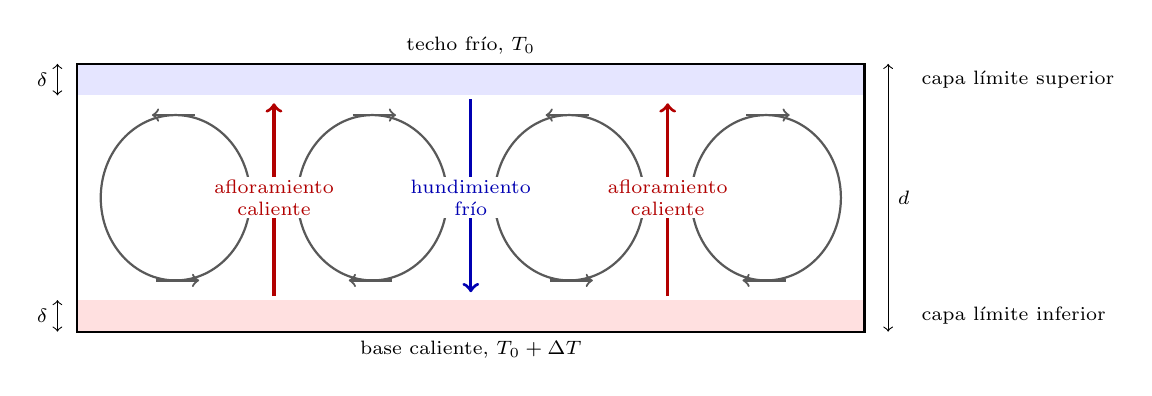
\begin{tikzpicture}[font=\scriptsize, x=1cm, y=1cm]
\fill[blue!10] (0,3.4) rectangle (10,3.0);
\fill[red!12] (0,0) rectangle (10,0.4);
\draw[thick] (0,0) rectangle (10,3.4);
\node[above] at (5,3.4) {techo frío, $T_0$};
\node[below] at (5,0) {base caliente, $T_0 + \Delta T$};
\foreach \c/\s in {1.25/1, 3.75/-1, 6.25/1, 8.75/-1} {
  \draw[gray!70!black, thick] (\c,1.7) ellipse[x radius=0.95, y radius=1.05];
  \draw[->, gray!70!black, thick] ({\c+0.25*\s},2.75) -- ({\c-0.3*\s},2.75);
  \draw[->, gray!70!black, thick] ({\c-0.25*\s},0.65) -- ({\c+0.3*\s},0.65);
}
\draw[->, red!70!black, very thick] (2.5,0.45) -- (2.5,2.9);
\draw[->, red!70!black, very thick] (7.5,0.45) -- (7.5,2.9);
\draw[->, blue!70!black, very thick] (5,2.95) -- (5,0.5);
\node[red!70!black, fill=white, inner sep=1pt, align=center] at (2.5,1.7) {afloramiento\\caliente};
\node[red!70!black, fill=white, inner sep=1pt, align=center] at (7.5,1.7) {afloramiento\\caliente};
\node[blue!70!black, fill=white, inner sep=1pt, align=center] at (5,1.7) {hundimiento\\frío};
\draw[<->] (10.3,0) -- (10.3,3.4) node[midway, right] {$d$};
\draw[<->] (-0.25,3.0) -- (-0.25,3.4) node[midway, left] {$\delta$};
\draw[<->] (-0.25,0) -- (-0.25,0.4) node[midway, left] {$\delta$};
\node[anchor=west] at (10.6,3.2) {capa límite superior};
\node[anchor=west] at (10.6,0.2) {capa límite inferior};
\end{tikzpicture}

\par\smallskip{\small Convección en una capa calentada desde abajo y enfriada desde
arriba. El calor atraviesa las capas límite delgadas, de espesor $\delta$, por
conducción; entre ellas, el interior bien mezclado lo transporta por flujo. Las láminas frías
se desprenden de la capa superior y se hunden; las calientes ascienden desde la
inferior.}\label{fig:b3:mantle-convection:cell}
\end{omfigure}

El manto también se calienta desde dentro, por la desintegración de elementos radiactivos,
y desde abajo, por el núcleo. Una capa calentada solo desde dentro no tiene
capa límite caliente en su base: su flujo está impulsado por láminas frías que se hunden desde la
parte superior, siendo el flujo ascendente un retorno amplio y pasivo. Las losas son láminas de ese tipo, y
las plumas necesitan el calor del núcleo.

\section{Capas límite y la intensidad de la convección}

\begin{definition}[Número de Nusselt]\label{def:b3:mantle-convection:nusselt}
El \emph{número de Nusselt}\index{número de Nusselt} de una capa en convección es el
flujo de calor que la atraviesa dividido por el flujo de calor que la conducción por sí sola transportaría
a través de la misma capa, $\mathrm{Nu} = q\,d/(k\,\Delta T)$.
\end{definition}

\begin{theorem}[Escalamiento de la convección por capa límite]\label{thm:b3:mantle-convection:scaling}
En una capa en convección con $\mathrm{Ra} \gg \mathrm{Ra}_c$, si cada capa límite térmica
crece hasta que su propio \omterm{def:b3:mantle-convection:rayleigh}{número de Rayleigh}, construido sobre su espesor
$\delta$ y la caída de temperatura $\Delta T/2$ a través de ella, alcanza
$\mathrm{Ra}_c$, entonces
\[
  \delta = d\Bigl(\frac{2\mathrm{Ra}_c}{\mathrm{Ra}}\Bigr)^{1/3},\qquad
  \mathrm{Nu} = \frac12\Bigl(\frac{\mathrm{Ra}}{2\mathrm{Ra}_c}\Bigr)^{1/3},
  \qquad
  u = \frac\kappa d\Bigl(\frac{\mathrm{Ra}}{2\mathrm{Ra}_c}\Bigr)^{2/3},
\]
donde $u$ es la escala de velocidad del flujo, definida exigiendo que la
capa crezca hasta $\delta$ mientras el fluido atraviesa la celda. Esta es la
\emph{escalamiento de la convección por capa límite}\index{escalamiento de la convección por capa límite}.
\end{theorem}

\begin{proof}
El interior está bien mezclado, a la temperatura media, así que cada capa límite
transporta la mitad de $\Delta T$. Su \omterm{def:b3:mantle-convection:rayleigh}{número de Rayleigh} es $\rho g\alpha(\Delta T/2)
\delta^3/(\kappa\eta) = \mathrm{Ra}\,(\delta/d)^3/2$; igualándolo a
$\mathrm{Ra}_c$ se obtiene $\delta$. El flujo de calor se conduce a través de la capa,
$q = k(\Delta T/2)/\delta$, luego $\mathrm{Nu} = qd/(k\Delta T) = d/(2\delta)$.
Una capa límite crece por difusión hasta el espesor $\delta$ en un tiempo
$\delta^2/\kappa$; el fluido de la parte superior atraviesa la celda, de anchura del orden de
$d$, en un tiempo $d/u$. Igualando los dos tiempos, $u = \kappa d/\delta^2 =
(\kappa/d)(d/\delta)^2$.
\end{proof}

El flujo de calor crece solo como la raíz cúbica de $\mathrm{Ra}$: una viscosidad
cien veces menor da menos de cinco veces más calor.
Con el $\mathrm{Ra} = \num{4.9e7}$ del manto, el escalamiento da $\delta \approx \qty{87}{km}$,
$\mathrm{Nu} \approx 17$, un flujo de calor de $\mathrm{Nu}\,k\Delta T/d \approx
\qty{26}{mW.m^{-2}}$ con $k = \qty{3.1}{W.m^{-1}.K^{-1}}$, y $u \approx
\qty{1.2}{cm/yr}$ (figura inferior). La capa límite tiene un espesor igual al de la
placa oceánica del \cref{ch:b3:lithosphere-thermal-models}, \qty{95}{km};
las velocidades medias cuadráticas de las placas actuales van de \qty{1.1}{cm/yr} (América del
Sur) a \qty{7.5}{cm/yr} (Cocos), \qty{4.4}{cm/yr} para la litosfera en
conjunto. El flujo de calor medio de la Tierra, \qty{92}{mW.m^{-2}}, es entre tres y cuatro
veces el del escalamiento: el calor producido dentro del manto, que una capa
calentada desde abajo omite, y las constantes de orden uno que el escalamiento
ignora; ambas pesan. Para una ley con una sola entrada, los órdenes de magnitud
son correctos: las placas son la capa límite superior de un manto con $\mathrm{Ra}
\sim 10^7$.
% ledger: nnr56:rms, b2dd10:continents, honda04:gdh1

\begin{omfigure}
\begin{tikzpicture}
\begin{groupplot}[group style={group size=1 by 2, vertical sep=2.5cm},
  omrecord, width=0.86\linewidth, height=0.40\linewidth, xmode=log, ymode=log,
  xmin=100, xmax=1e10, xlabel={Número de Rayleigh $\mathrm{Ra}$}]
\nextgroupplot[ylabel={Número de Nusselt}, ymin=0.3, ymax=300,
  title={(a) flujo de calor, en unidades del flujo conductivo}, title style={font=\small}]
% computed in figdata/bachelor-3/convection_scaling.py; ledger: data:prem, honda04:gdh1
\addplot[omDef, thick] table[x=ra, y=nu] {figdata/out/bachelor-3-convection_scaling-conduction.dat};
\addplot[red!70!black, thick] table[x=ra, y=nu] {figdata/out/bachelor-3-convection_scaling-scaling.dat};
\addplot[gray, densely dashed, unbounded coords=jump] table[x=ra, y=y] {figdata/out/bachelor-3-convection_scaling-band.dat};
\draw[gray, densely dotted] (axis cs:657.5,0.3) -- (axis cs:657.5,1);
\node[font=\scriptsize, anchor=west] at (axis cs:700,0.45) {$\mathrm{Ra}_c$};
\node[font=\scriptsize, anchor=south west, omDef] at (axis cs:115,1.08) {conducción};
\node[font=\scriptsize, anchor=north west, red!70!black] at (axis cs:3e4,0.95) {$\tfrac12(\mathrm{Ra}/2\mathrm{Ra}_c)^{1/3}$};
\node[font=\scriptsize, fill=white, inner sep=1pt] at (axis cs:1.55e7,120) {manto};
\nextgroupplot[ylabel={velocidad (\unit{cm/yr})}, ymin=1e-3, ymax=100,
  title={(b) escala de velocidad para $d = \qty{2891}{km}$}, title style={font=\small}]
\addplot[red!70!black, thick] table[x=ra, y=u] {figdata/out/bachelor-3-convection_scaling-scaling.dat};
\addplot[gray, densely dashed, unbounded coords=jump] table[x=ra, y=y] {figdata/out/bachelor-3-convection_scaling-band.dat};
\addplot[blue!70, thick, dash dot, unbounded coords=jump] table[x=ra, y=u] {figdata/out/bachelor-3-convection_scaling-plates.dat};
\node[font=\scriptsize, anchor=south west, blue!60!black] at (axis cs:150,7.6) {placa más rápida};
\node[font=\scriptsize, anchor=north west, blue!60!black] at (axis cs:150,1.0) {placa más lenta};
\node[font=\scriptsize, fill=white, inner sep=1pt] at (axis cs:1.55e7,0.004) {manto};
\end{groupplot}
\end{tikzpicture}

\par\smallskip{\small Escalamiento de la convección. (a) Por debajo de $\mathrm{Ra}_c$ la capa
conduce ($\mathrm{Nu} = 1$); muy por encima, la ley de capa límite, trazada
desde $\mathrm{Ra} = 16\,\mathrm{Ra}_c \approx \num{1.1e4}$, donde da $\mathrm{Nu} = 1$ (entre medias,
la convección se instala gradualmente). (b) La escala de velocidad
para la profundidad del manto y $\kappa = \qty{e-6}{m^2.s^{-1}}$, con el
intervalo de velocidades actuales de las placas (trazo punto-raya). Las líneas discontinuas acotan el
\omterm{def:b3:mantle-convection:rayleigh}{número de Rayleigh} del manto para viscosidades de \num{e22} y \qty{e21}{Pa.s}.}\label{fig:b3:mantle-convection:scaling}
\end{omfigure}

\section{Las fuerzas sobre una placa}

Una placa se mueve a velocidad constante: las fuerzas sobre ella se equilibran. Tres la impulsan o la
frenan desde sus bordes y su base (figura inferior). La fuerza que la
losa que se hunde ejerce sobre su placa, el tirón de la losa, procede del exceso de densidad de
una losa fría en el manto más caliente. El empuje de la dorsal, el que ejerce la dorsal alta y caliente
sobre la placa más fría contigua, se deduce del \omterm{def:b3:lithosphere-thermal-models:half-space}{modelo de enfriamiento de semiespacio} expuesto en el
\cref{ch:b3:lithosphere-thermal-models}.

\begin{omfigure}
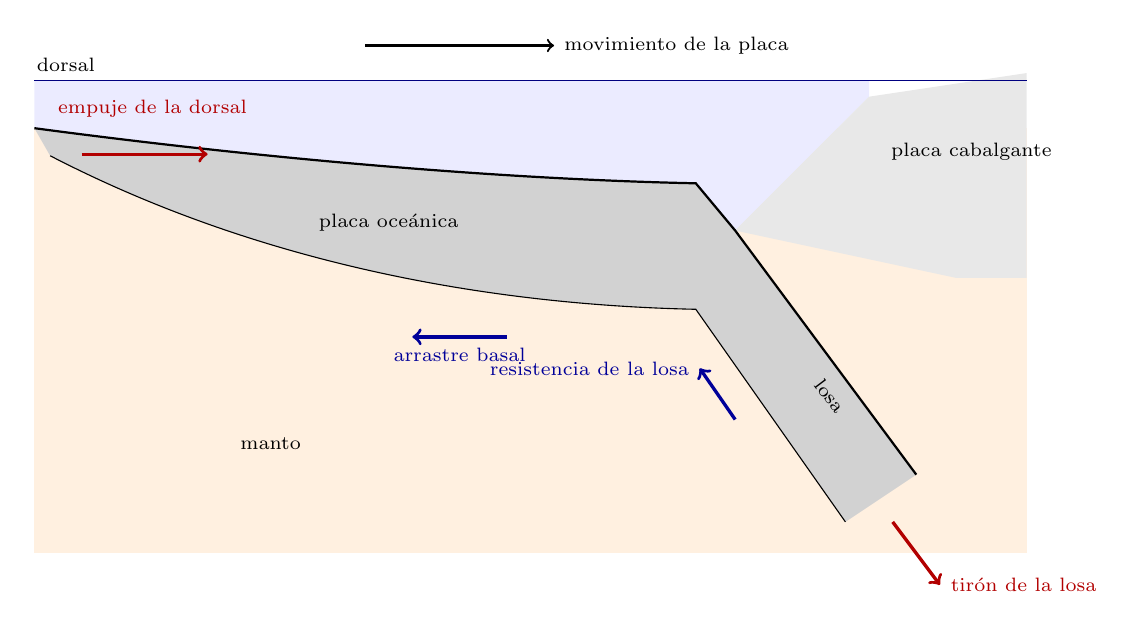
\begin{tikzpicture}[font=\scriptsize, x=1cm, y=1cm]
\fill[orange!12] (0,-0.6) rectangle (12.6,-6.0);
\fill[blue!8] (0,0) -- (0,-0.6) .. controls (3,-1.0) and (6,-1.25) .. (8.4,-1.3) -- (8.9,-1.9) -- (10.6,-0.2) -- (10.6,0) -- cycle;
\fill[gray!35] (0,-0.6) .. controls (3,-1.0) and (6,-1.25) .. (8.4,-1.3) -- (8.9,-1.9) -- (11.2,-5.0) -- (10.3,-5.6) -- (8.4,-2.9) .. controls (6,-2.85) and (3,-2.4) .. (0.2,-0.95) -- cycle;
\fill[gray!18] (10.6,-0.2) -- (12.6,0.1) -- (12.6,-2.5) -- (11.7,-2.5) -- (8.9,-1.9) -- cycle;
\draw[thick] (0,-0.6) .. controls (3,-1.0) and (6,-1.25) .. (8.4,-1.3) -- (8.9,-1.9) -- (11.2,-5.0);
\draw (0.2,-0.95) .. controls (3,-2.4) and (6,-2.85) .. (8.4,-2.9) -- (10.3,-5.6);
\draw[blue!50!black] (0,0) -- (12.6,0);
\node at (0.4,0.2) {dorsal};
\node at (4.5,-1.8) {placa oceánica};
\node at (11.9,-0.9) {placa cabalgante};
\node[rotate=-53] at (10.1,-4.0) {losa};
\node at (3,-4.6) {manto};
\draw[->, very thick, red!70!black] (0.6,-0.93) -- (2.2,-0.93);
\node[red!70!black] at (1.5,-0.35) {empuje de la dorsal};
\draw[->, very thick, red!70!black] (10.9,-5.6) -- (11.5,-6.4) node[right] {tirón de la losa};
\draw[->, very thick, blue!60!black] (6.0,-3.25) -- (4.8,-3.25) node[below, pos=0.5] {arrastre basal};
\draw[->, very thick, blue!60!black] (8.9,-4.3) -- (8.45,-3.65) node[left] {resistencia de la losa};
\draw[->, thick] (4.2,0.45) -- (6.6,0.45) node[right] {movimiento de la placa};
\end{tikzpicture}

\par\smallskip{\small Las fuerzas sobre una placa oceánica: el empuje de la dorsal y el tirón de la losa
impulsan la placa (en rojo); el arrastre en su base, donde la placa se mueve más deprisa que el manto
subyacente, y la resistencia viscosa del manto a la losa que se hunde se oponen a ella
(en azul).}\label{fig:b3:mantle-convection:forces}
\end{omfigure}

\begin{proposition}[Fuerza de empuje de la dorsal]\label{prop:b3:mantle-convection:ridge-push}
En el \omterm{def:b3:lithosphere-thermal-models:half-space}{modelo de enfriamiento de semiespacio}, con temperatura del manto $T_m$, temperatura superficial
$T_0$ y compensación isostática, la fuerza horizontal por unidad
de longitud de dorsal que la columna en la dorsal ejerce sobre la placa de edad $t$,
la \emph{fuerza de empuje de la dorsal}\index{fuerza de empuje de la dorsal}, es
\[
  F_{rp} = g\rho_m\alpha(T_m - T_0)\kappa t\Bigl[1 + \frac{2\rho_m\alpha(T_m
  - T_0)}{\pi(\rho_m - \rho_w)}\Bigr].
\]
\end{proposition}

\begin{proof}
Sea $y$ la profundidad bajo el fondo marino en la dorsal, $w$ la subsidencia del
fondo de edad $t$, $\theta(z) = T_m - T(z)$ el déficit de temperatura en el
en la profundidad $z = y - w$ de su placa, y $\Theta(z) = \int_0^z\theta$. La
columna de la dorsal contiene manto de densidad $\rho_m$ desde $y = 0$; la columna antigua
contiene agua hasta $w$, luego placa de densidad $\rho_m(1 + \alpha\theta)$. Las
presiones litostáticas difieren en $P_r - P_t = (\rho_m - \rho_w)gy$ para $y < w$,
y por debajo,
\[
  P_r - P_t = (\rho_m - \rho_w)gw - \rho_mg\alpha\,\Theta(z)
  = \rho_mg\alpha\bigl(\Theta(\infty) - \Theta(z)\bigr),
\]
por isostasia, $(\rho_m - \rho_w)w = \rho_m\alpha\Theta(\infty)$. La fuerza es la
integral de la diferencia de presión en profundidad; integrando la segunda parte por
partes,
\[
  F_{rp} = \tfrac12(\rho_m - \rho_w)gw^2 + \rho_mg\alpha\int_0^\infty
  z\,\theta(z)\,\mathrm dz .
\]
Para el semiespacio, $\theta = (T_m - T_0)\operatorname{erfc}(z/2\sqrt{\kappa
t})$ y $\int_0^\infty x\operatorname{erfc}x\,\mathrm dx = 1/4$, así la
integral es $(T_m - T_0)\kappa t$; y $w = 2\rho_m\alpha(T_m -
T_0)\sqrt{\kappa t/\pi}/(\rho_m - \rho_w)$. Sumando los dos términos se obtiene la
fórmula.
\end{proof}

El empuje de la dorsal crece linealmente con la edad: no es un empuje en el eje sino un
gradiente de presión repartido por toda la placa que se enfría. Con los valores del
\cref{ch:b3:lithosphere-thermal-models}, el corchete vale 1.04 y $F_{rp} =
\qty{3.8e12}{N.m^{-1}}$ a \qty{100}{Myr}. En el modelo de placa deja de crecer
con la profundidad, hacia \qty{2.3e12}{N.m^{-1}} (figura inferior). El tirón de la losa es
mayor: una losa de \qty{95}{km} de espesor, en promedio $(T_m - T_0)/2$ más fría que el
manto, y por tanto más densa en $\rho_m\alpha(T_m - T_0)/2 \approx
\qty{74}{kg.m^{-3}}$, que cuelga hasta \qty{670}{km}, pesa
\qty{4.6e13}{N.m^{-1}} más que el manto que desplaza, doce veces el
empuje de la dorsal. Gran parte de ese peso se invierte en el manto viscoso que se opone al
hundimiento de la losa, y solo una parte llega a la placa.
% ledger: honda04:gdh1, data:prem

\begin{omfigure}
\begin{tikzpicture}
\begin{axis}[omrecord, width=0.8\linewidth, height=0.42\linewidth,
  xmin=0, xmax=160, ymin=0, ymax=6.5, xlabel={edad del fondo marino (Myr)},
  ylabel={$F_{rp}$ (\qty{e12}{N.m^{-1}})},
  legend cell align=left,
  legend style={font=\scriptsize, at={(0.03,0.97)}, anchor=north west}]
% computed in figdata/bachelor-3/ridge_push.py; ledger: honda04:gdh1
\addplot[omDef, thick] table[x=t, y=hs] {figdata/out/bachelor-3-ridge_push-force.dat};
\addlegendentry{semiespacio}
\addplot[red!70!black, thick, densely dashed] table[x=t, y=pl] {figdata/out/bachelor-3-ridge_push-force.dat};
\addlegendentry{placa, $L = \qty{95}{km}$}
\end{axis}
\end{tikzpicture}

\par\smallskip{\small \omterm{prop:b3:mantle-convection:ridge-push}{Fuerza de empuje de la dorsal} frente a la edad de la placa, a partir de los
dos modelos de enfriamiento del \cref{ch:b3:lithosphere-thermal-models}, mediante
integración numérica de la diferencia de presión (la curva de semiespacio es la
forma cerrada de la proposición).}\label{fig:b3:mantle-convection:ridge-push}
\end{omfigure}

\begin{definition}[Arrastre basal]\label{def:b3:mantle-convection:basal-drag}
El \emph{arrastre basal}\index{arrastre basal} es la fuerza de cizalla por unidad de superficie que el
manto bajo una placa ejerce sobre la base de la placa. Para una placa que se mueve a velocidad $u$
sobre una capa de espesor $h$ y viscosidad $\eta$ cuya base está en reposo, es
$\eta u/h$, opuesta al movimiento; impulsa la placa donde el manto subyacente
se mueve más deprisa que la placa.
\end{definition}

Qué fuerzas importan puede leerse en las propias placas. El balance de momentos
en cada placa, ajustado a los movimientos de las placas, indica que las fuerzas que actúan sobre la
losa que se hunde controlan la velocidad de las placas oceánicas y son unas diez veces
más intensas que cualesquiera otras, y que la resistencia en la base es mayor bajo los
continentes que bajo los océanos. Las velocidades concuerdan: las placas más rápidas, Cocos a
\qty{75}{mm/yr}, Nazca a 70 y el Pacífico a \qty{66}{mm/yr}, son placas oceánicas
cuyos bordes se hunden en fosas largas; las más lentas portan grandes continentes,
Eurasia a 23, América del Norte a 20, América del Sur a \qty{11}{mm/yr}.
% ledger: fu75:slab-pull, nnr56:rms

\section{Plumas}

Las láminas de material caliente que ascienden desde la base del manto se agrupan en columnas: las plumas del manto
tratadas en el volumen de primer año, con una cabeza grande y una cola delgada (figura de más abajo).
El abombamiento de un punto caliente, una elevación amplia del fondo marino alrededor y aguas abajo de
los volcanes, mide cuánta flotabilidad aporta su pluma.

\begin{definition}[Flujo de flotabilidad de la pluma]\label{def:b3:mantle-convection:buoyancy-flux}
El \emph{flujo de flotabilidad de la pluma}\index{flujo de flotabilidad de la pluma} $B$ es el déficit de masa,
respecto del manto circundante, que una pluma transporta hacia arriba por unidad de
tiempo; para una pluma de flujo volumétrico $Q_v$ y exceso de temperatura $\Delta T$,
$B = \rho\alpha\,\Delta T\,Q_v$.
\end{definition}

\begin{proposition}[Flotabilidad a partir de un abombamiento]\label{prop:b3:mantle-convection:swell}
Si una placa que se mueve a la velocidad $u$ sobre una pluma arrastra un abombamiento de
área de sección transversal $A$ a lo largo de la traza, sostenido isostáticamente por el material de la pluma
situado debajo, el \omterm{def:b3:mantle-convection:buoyancy-flux}{flujo de flotabilidad de la pluma} es
\[
  B = (\rho_m - \rho_w)\,A\,u .
\]
\end{proposition}

\begin{proof}
Por isostasia, una rebanada de abombamiento de longitud unitaria a lo largo de la traza, que eleva
el fondo marino sobre el área $A$ de la sección transversal y sustituye agua por
roca, se sostiene mediante un déficit de masa $(\rho_m - \rho_w)A$ en la columna situada debajo.
La placa arrastra la rebanada a la velocidad $u$, de modo que en estado estacionario la
pluma debe suplir el déficit correspondiente a una longitud $u$ de nuevo abombamiento por unidad de tiempo.
\end{proof}

A partir de las secciones transversales de los abombamientos, los flujos de flotabilidad de los puntos calientes varían en
un factor de veinte: Hawái, el mayor, \qty{8.7}{Mg/s}; Islandia
\qty{1.4}{Mg/s}; 37 puntos calientes en conjunto, unos \qty{50}{Mg/s}. Cada kilogramo de
flotabilidad equivale a $c_p/\alpha$ julios de calor en exceso, de modo que el flujo de calor es $c_pB/\alpha$;
con $c_p = k/(\rho_m\kappa) = \qty{1170}{J.kg^{-1}.K^{-1}}$ y $\alpha =
\qty{3.1e-5}{K^{-1}}$, los 37 puntos calientes transportan unos \qty{1.9}{TW}, o
\qty{3.7}{mW.m^{-2}} sobre los \qty{5.1e14}{m^2} de la Tierra, cerca de los
\qty{4}{mW.m^{-2}} publicados junto con los flujos: unos pocos por ciento de los
\qty{47}{TW} que pierde la Tierra. Las plumas son el socio menor del
balance de calor; las placas transportan el resto.
% ledger: sleep90:flux, b2dd10:half-space, honda04:gdh1

\begin{omfigure}
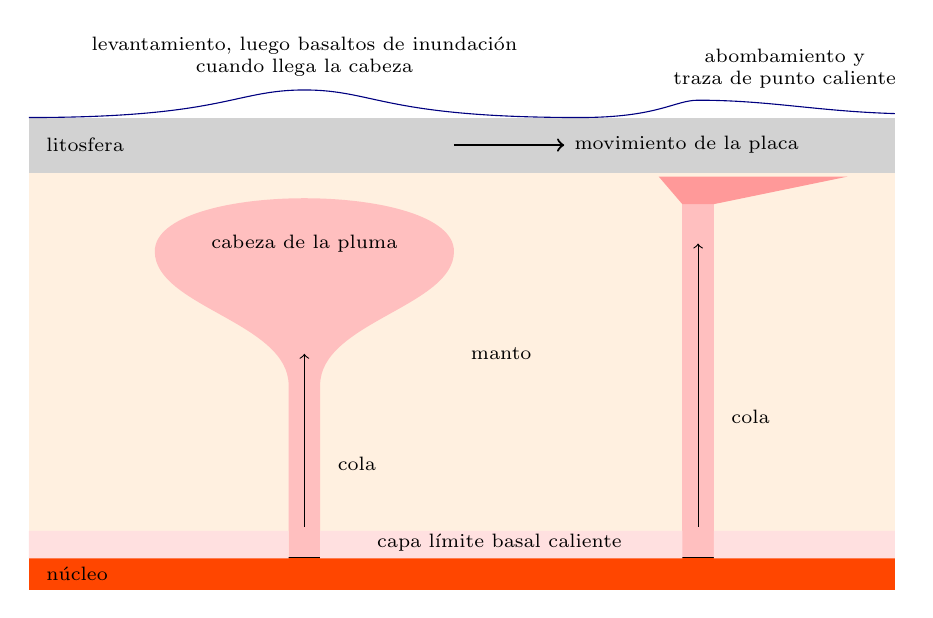
\begin{tikzpicture}[font=\scriptsize, x=1cm, y=1cm]
\fill[orange!12] (0,0) rectangle (11,-5.6);
\fill[gray!35] (0,0) -- (11,0) -- (11,-0.7) -- (0,-0.7) -- cycle;
\fill[red!25] (3.3,-5.6) -- (3.3,-3.4) .. controls (3.3,-2.6) and (1.6,-2.4) .. (1.6,-1.7)
  .. controls (1.6,-0.8) and (5.4,-0.8) .. (5.4,-1.7) .. controls (5.4,-2.4) and (3.7,-2.6) .. (3.7,-3.4) -- (3.7,-5.6) -- cycle;
\fill[red!25] (8.3,-5.6) -- (8.3,-0.75) -- (8.7,-0.75) -- (8.7,-5.6) -- cycle;
\fill[red!40] (8.0,-0.75) -- (8.3,-1.1) -- (8.7,-1.1) -- (10.4,-0.75) -- cycle;
\draw[thick] (0,-5.6) -- (11,-5.6);
\fill[red!45!orange] (0,-5.6) rectangle (11,-6.0);
\fill[red!12] (0,-5.6) rectangle (3.3,-5.25) (3.7,-5.6) rectangle (8.3,-5.25) (8.7,-5.6) rectangle (11,-5.25);
\node[anchor=west] at (0.1,-5.8) {núcleo};
\node at (3.5,-1.6) {cabeza de la pluma};
\node[anchor=west] at (3.8,-4.4) {cola};
\node[anchor=west] at (8.8,-3.8) {cola};
\node[anchor=west] at (0.1,-0.35) {litosfera};
\node at (6.0,-3.0) {manto};
\draw[->] (3.5,-5.2) -- (3.5,-3.0);
\draw[->] (8.5,-5.2) -- (8.5,-1.6);
\draw[->, thick] (5.4,-0.35) -- (6.8,-0.35) node[right] {movimiento de la placa};
\draw[blue!50!black] (0,0) .. controls (2.5,0) and (2.6,0.35) .. (3.5,0.35) .. controls (4.4,0.35) and (4.5,0) .. (7,0) .. controls (8,0) and (8.2,0.22) .. (8.5,0.22) .. controls (9.4,0.22) and (10,0.08) .. (11,0.05);
\node[above, align=center] at (3.5,0.4) {levantamiento, luego basaltos de inundación\\cuando llega la cabeza};
\node[above, align=center] at (9.6,0.25) {abombamiento y\\traza de punto caliente};
\node[anchor=west] at (4.3,-5.4) {capa límite basal caliente};
\end{tikzpicture}

\par\smallskip{\small Una pluma joven (izquierda) asciende como una cabeza grande alimentada por una cola delgada;
cuando la cabeza se extiende bajo la litosfera, la superficie se eleva y pueden erupcionar basaltos de
inundación. Una pluma más antigua (derecha) es una cola bajo una placa en movimiento,
que alimenta un abombamiento y una traza de punto caliente. No a
escala.}\label{fig:b3:mantle-convection:plume}
\end{omfigure}

Una cabeza de pluma es una esfera de manto flotante que asciende a través del manto viscoso:
la ley de Stokes de la física, $v = 2\Delta\rho\,ga^2/(9\eta)$, da su velocidad en orden de
magnitud: una fracción de metro al año para una cabeza de unos pocos cientos de kilómetros
de diámetro (ejercicio 8), de modo que cruza el manto en millones de años.

\section{Ajuste isostático glaciar y viscosidad del manto}\label{sec:b3:mantle-convection:gia}

\begin{definition}[Ajuste isostático glaciar, viscosidad del manto]\label{def:b3:mantle-convection:gia}
El \emph{ajuste isostático glaciar}\index{ajuste isostático glaciar} (GIA, por sus siglas en inglés)
es la deformación lenta de la Tierra sólida, y el cambio de su campo gravitatorio
y del nivel del mar, a medida que regresa hacia el equilibrio isostático tras
crecer o fundirse un casquete de hielo. La \emph{viscosidad del manto}\index{viscosidad del manto}
es la viscosidad efectiva $\eta$ que relaciona la fluencia lenta y estacionaria del
manto con los esfuerzos que la impulsan, en escalas de miles de años o más.
\end{definition}

Cuando se funde un casquete de hielo, la depresión que deja queda fuera del
equilibrio isostático: bajo ella, la presión del manto es menor que en los alrededores, y
el manto fluye hacia dentro para elevar de nuevo el suelo. Hoy la costa del golfo de Botnia
se eleva hasta \qty{10.3}{mm/yr}, cerca de Umeå; la bahía de Hudson, unos
\qty{10}{mm/yr}, donde el hielo era más grueso, mientras que el terreno al sur de los Grandes
Lagos se hunde entre 1 y \qty{2}{mm/yr}, a medida que se hunde el abombamiento que el hielo había elevado
a su alrededor. En las costas, antiguas líneas de costa se encuentran ahora por encima del mar, las
playas levantadas del recuadro de campo de más abajo.
% ledger: vestol19:umea, sella07:gia

\begin{theorem}[Relajación de un semiespacio viscoso]\label{thm:b3:mantle-convection:relaxation}
Una depresión $w(x, t) = w_m(t)\cos(2\pi x/\lambda)$ de la superficie de un
semiespacio de viscosidad uniforme $\eta$ y densidad $\rho$, sin carga,
decae como $w_m(t) = w_m(0)e^{-t/\tau}$ con
\[
  \tau = \frac{4\pi\eta}{\rho g\lambda} .
\]
\end{theorem}

\begin{proof}
Tómese $z$ hacia abajo, $k = 2\pi/\lambda$, y búsquese un flujo de Stokes que decaiga
con la profundidad, con velocidad vertical (hacia abajo) $v = (C + Dkz)e^{-kz}\cos kx$.
La incompresibilidad da la velocidad horizontal $u = -(D - C - Dkz)e^{-kz}\sin
kx$. Estas funciones satisfacen $\nabla^4 = 0$, como lo hace todo flujo de Stokes
en dos dimensiones. La superficie libre no soporta esfuerzo de cizalla: $\partial u/\partial
z + \partial v/\partial x = 2k(D - C)\sin kx = 0$ en $z = 0$, así que $D = C$, y
\[
  v = C(1 + kz)e^{-kz}\cos kx,\quad u = Ckze^{-kz}\sin kx,\quad
  p = 2\eta Cke^{-kz}\cos kx,
\]
la presión se deduce de $\partial p/\partial x = \eta\nabla^2u = -2\eta
Ck^2e^{-kz}\sin kx$ (y $\partial p/\partial z = \eta\nabla^2v$ se comprueba). En la
superficie $\partial v/\partial z = 0$, así que el esfuerzo normal allí es $-p$. Bajo
una depresión $w$, el peso de la roca ausente reduce la presión en $\rho
gw$: $p(0) = -\rho gw$, luego $2\eta Ck = -\rho gw_m$. La superficie se mueve con el
fluido: $\mathrm dw_m/\mathrm dt = v(0) = C = -\rho gw_m/(2\eta k)$, cuya
solución decae con $\tau = 2\eta k/(\rho g) = 4\pi\eta/(\rho g\lambda)$.
\end{proof}

\begin{definition}[Tiempo de relajación isostática]\label{def:b3:mantle-convection:relaxation-time}
El \emph{tiempo de relajación isostática}\index{tiempo de relajación isostática} $\tau$ de
una carga de escala horizontal $\lambda$ es el tiempo en el que su desviación del
equilibrio isostático decae en un factor $e$.
\end{definition}

Un semiespacio uniforme relaja más rápido las depresiones amplias que las estrechas, y el
flujo bajo una carga de longitud de onda $\lambda$ decae con la profundidad como $e^{-kz}$, sobre
una profundidad $\lambda/2\pi$: un casquete de hielo grande agita el manto en profundidad, un lago pequeño
solo su parte superior. Para una depresión de \qty{3000}{km} de ancho y $\eta =
\qty{e21}{Pa.s}$, con $\rho = \qty{3300}{kg.m^{-3}}$, $\tau = \qty{4.1}{kyr}$
(figura siguiente): tras diez mil años, queda $e^{-2.4} = \qty{9}{\percent}$ de
la depresión, y como $\dot w = -w/\tau$, un levantamiento de
\qty{10}{mm/yr} significa que aún quedan por llegar unos \qty{40}{m} de ascenso.

\begin{omfigure}
\begin{tikzpicture}
\begin{groupplot}[group style={group size=1 by 2, vertical sep=2.5cm},
  omrecord, width=0.86\linewidth, height=0.38\linewidth]
\nextgroupplot[xmin=0, xmax=20, ymin=0, ymax=1.05, xlabel={tiempo desde que se fundió el hielo (kyr)},
  ylabel={$w_m(t)/w_m(0)$}, title={(a) decaimiento de una depresión de \qty{3000}{km} de ancho},
  title style={font=\small}, legend style={font=\scriptsize, at={(0.98,0.97)}, anchor=north east}]
% computed in figdata/bachelor-3/gia_relaxation.py; ledger: mitrovica96:haskell, milne04:bifrost
\addplot[red!70!black, thick, densely dashed] table[x=t, y=f20] {figdata/out/bachelor-3-gia_relaxation-decay.dat};
\addlegendentry{$\eta = \qty{e20}{Pa.s}$}
\addplot[omDef, thick] table[x=t, y=f21] {figdata/out/bachelor-3-gia_relaxation-decay.dat};
\addlegendentry{$\eta = \qty{e21}{Pa.s}$}
\addplot[black, thick, densely dotted] table[x=t, y=f22] {figdata/out/bachelor-3-gia_relaxation-decay.dat};
\addlegendentry{$\eta = \qty{e22}{Pa.s}$}
\nextgroupplot[xmode=log, ymode=log, xmin=100, xmax=1e4, ymin=0.01, ymax=1000,
  xlabel={longitud de onda $\lambda$ (km)}, ylabel={$\tau$ (kyr)},
  title={(b) tiempo de relajación frente a la longitud de onda}, title style={font=\small}]
\addplot[red!70!black, thick, densely dashed] table[x=lam, y=t20] {figdata/out/bachelor-3-gia_relaxation-tau.dat};
\addplot[omDef, thick] table[x=lam, y=t21] {figdata/out/bachelor-3-gia_relaxation-tau.dat};
\addplot[black, thick, densely dotted] table[x=lam, y=t22] {figdata/out/bachelor-3-gia_relaxation-tau.dat};
\end{groupplot}
\end{tikzpicture}

\par\smallskip{\small Relajación de un semiespacio viscoso uniforme ($\rho =
\qty{3300}{kg.m^{-3}}$, $g = \qty{9.8}{m.s^{-2}}$) para tres viscosidades. (a) La
fracción de la depresión que queda con el tiempo. (b) El tiempo de relajación
$4\pi\eta/(\rho g\lambda)$, más largo para cargas estrechas.}\label{fig:b3:mantle-convection:gia}
\end{omfigure}

El manto real no es uniforme, y su rebote se interpreta con modelos que lo estratifican
y añaden una litosfera elástica, que sostiene las cargas estrechas por flexión. La
primera estimación, a partir del rebote de Fennoscandia, dio \qty{e21}{Pa.s}, y el
decaimiento del levantamiento en el río Angerman, en Suecia, y en Richmond Gulf, en la
bahía de Hudson, da un promedio de 0.65 a \qty{1.1e21}{Pa.s} desde la base de la
litosfera hasta unos \qty{1400}{km}, con el manto superior unas diez veces
menos viscoso que el inferior. Las inversiones de las tasas de levantamiento GNSS de
Fennoscandia dan \omterm{def:b3:mantle-convection:gia}{viscosidades del manto} superior de \num{5e20} a \qty{e21}{Pa.s}
en un estudio y de \num{3.4e20} a \qty{5.0e20}{Pa.s} en otro, \omterm{def:b3:mantle-convection:gia}{viscosidades del manto}
inferior de \num{5e21} a \qty{5e22}{Pa.s}, y una litosfera de entre 93 y
\qty{110}{km} de espesor. Las estimaciones difieren en factores de dos o tres, pero
coinciden en el orden de magnitud y en el aumento con la profundidad.
% ledger: mitrovica96:haskell, milne04:bifrost, zhao12:fenno

\begin{definition}[Tiempo de Maxwell]\label{def:b3:mantle-convection:maxwell}
El \emph{tiempo de Maxwell}\index{tiempo de Maxwell} de un material de viscosidad $\eta$
y módulo de cizalla $\mu$ es $\tau_M = \eta/\mu$: las cargas aplicadas durante mucho menos que
$\tau_M$ encuentran un sólido elástico, las aplicadas durante mucho más un fluido viscoso.
\end{definition}

Con $\mu = \rho v_S^2 = \qty{7.7e10}{Pa}$ a \qty{300}{km} en PREM y $\eta =
\qty{e21}{Pa.s}$, $\tau_M = \qty{1.3e10}{s}$, unos cuatrocientos años. Una
onda sísmica, que dura segundos, atraviesa un manto elástico; una edad de hielo y la
convección deforman un fluido. La misma roca es ambas cosas, según el tiempo durante el que
se la empuje.
% ledger: data:prem

\begin{inthefield}[Playas levantadas]
\begin{minipage}[t]{0.55\linewidth}\vspace{0pt}
En las costas de tierras antes glaciares, un geomorfólogo encuentra el antiguo trabajo del
mar varado tierra adentro: crestas de guijarros redondeados, muescas y plataformas
planas talladas por las olas, hoy por encima del alcance de las
mareas más altas actuales, a veces en una escalera de varios niveles. Cada nivel fue una línea de
costa cuando el mar estaba allí; la tierra se ha elevado desde entonces. Las conchas y la madera flotante
de las playas antiguas se datan por radiocarbono, y las alturas de los niveles datados,
nivelados a un punto de referencia, dan el levantamiento frente al tiempo. Trazada a lo largo de una costa,
una línea de costa antigua resulta tener pendiente, más alta donde el hielo era más grueso: la
inclinación refleja la forma del rebote.
\end{minipage}\hfill
\begin{minipage}[t]{0.42\linewidth}\vspace{0pt}
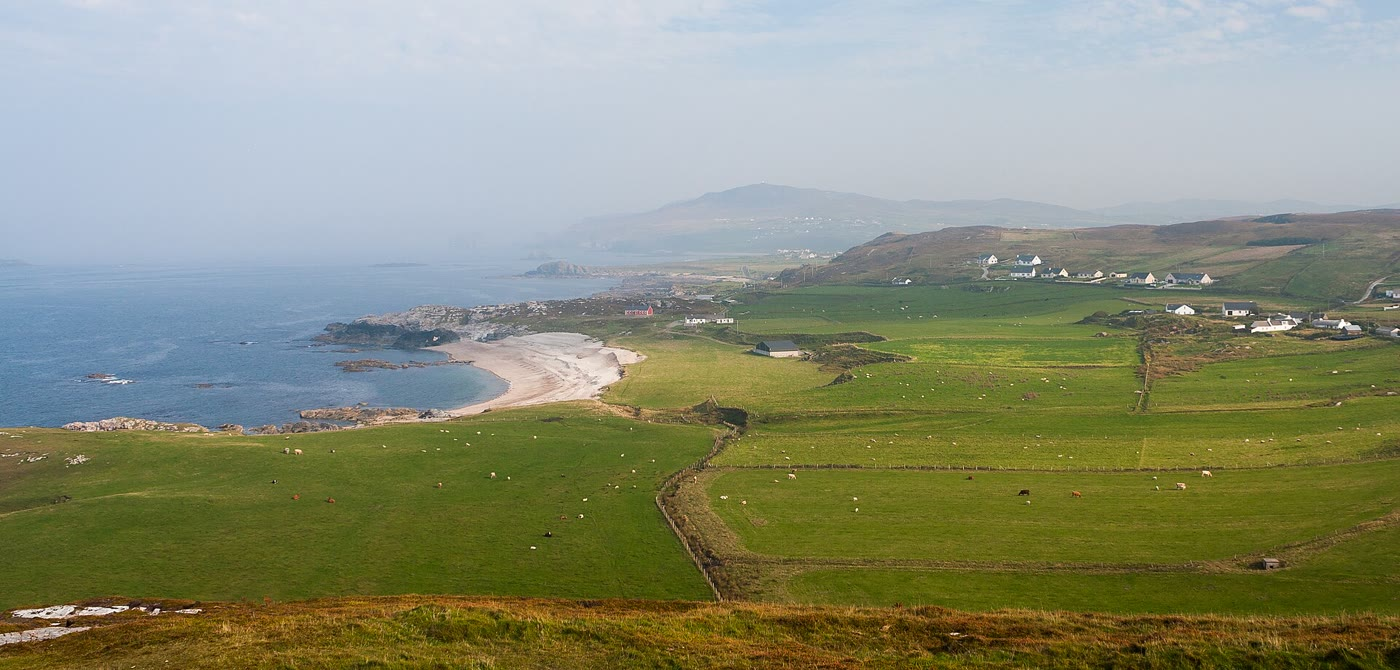
\includegraphics[width=\linewidth]{images/book5/b3-raised-beach-malin.jpg}

{\scriptsize Las playas levantadas de Ballyhillin, Malin Head, en el norte de
Irlanda: crestas de guijarros de antiguas líneas de costa elevadas sobre el mar a medida que la
tierra se alzó tras la fusión de su casquete de hielo. Foto A.~F.~Borchert, CC BY-SA 4.0.}
\end{minipage}
\end{inthefield}
% ledger: photo:b3-raised-beach

\section{Convección de todo el manto y su estructura profunda}

¿Convecta el manto como una sola capa o como dos, por encima y por debajo de la
discontinuidad de \qty{670}{km}? La tomografía (véase el \cref{ch:b3:seismology-imaging})
responde en parte: algunas losas se aplanan por encima de la discontinuidad, mientras que otras se hunden
a través de ella hasta el manto inferior, de modo que la masa la atraviesa y las dos capas no están
aisladas entre sí. El aumento de la viscosidad con la profundidad hace que el manto inferior fluya con mayor lentitud,
y las losas se ralenticen y engrosen al entrar en él.

En la base del manto, la tomografía muestra dos amplias regiones de baja velocidad de las ondas S,
bajo África y bajo el Pacífico, las grandes provincias de baja velocidad de cizalla
(LLSVP). Probablemente son químicamente distintas del manto que tienen encima
y más densas: acumulaciones y no plumas calientes. Las grandes provincias ígneas y
las kimberlitas de los últimos cientos de millones de años entraron en erupción sobre todo encima de sus
márgenes, como si las plumas ascendieran desde los bordes de las acumulaciones, allí donde la capa límite
caliente de la base del manto es empujada contra ellas.
% ledger: st12:llsvp

\section{Ejercicios}

\begin{exercise}[$\star$]\label{exo:b3:mantle-convection:1}
Calcúlese el \omterm{def:b3:mantle-convection:rayleigh}{número de Rayleigh} de una capa del manto superior de \qty{670}{km} de espesor con
$\rho = \qty{3500}{kg.m^{-3}}$, $g = \qty{9.9}{m.s^{-2}}$, $\alpha =
\qty{3e-5}{K^{-1}}$, $\Delta T = \qty{1000}{K}$, $\kappa =
\qty{e-6}{m^2.s^{-1}}$ y $\eta = \qty{5e20}{Pa.s}$. ¿Cuántas veces supera al valor crítico
para contornos de deslizamiento libre?
\end{exercise}

\begin{exercise}[$\star$]\label{exo:b3:mantle-convection:2}
Calcúlese el \omterm{def:b3:mantle-convection:maxwell}{tiempo de Maxwell} de un manto de viscosidad \qty{e21}{Pa.s} y de módulo de
cizalla \qty{7.7e10}{Pa}, en años. ¿Responde el manto de forma elástica o viscosa a la marea
terrestre semidiurna, a la fusión de un casquete de hielo y al
hundimiento de una losa?
\end{exercise}

\begin{exercise}[$\star$]\label{exo:b3:mantle-convection:3}
Con $\eta = \qty{e21}{Pa.s}$, $\rho = \qty{3300}{kg.m^{-3}}$ y $g =
\qty{9.8}{m.s^{-2}}$, calcúlese el tiempo de relajación de un semiespacio uniforme para
cargas de longitud de onda de 1000 y \qty{3000}{km}. ¿Cuál se recupera más rápido?
\end{exercise}

\begin{exercise}[$\star$]\label{exo:b3:mantle-convection:4}
Con $g = \qty{9.8}{m.s^{-2}}$, $\rho_m = \qty{3300}{kg.m^{-3}}$, $\rho_w =
\qty{1030}{kg.m^{-3}}$, $\alpha = \qty{3.1e-5}{K^{-1}}$, $T_m - T_0 =
\qty{1450}{K}$, $\kappa = \qty{0.8e-6}{m^2.s^{-1}}$ y \qty{1}{Myr} $=
\qty{3.156e13}{s}$, calcúlese la \omterm{prop:b3:mantle-convection:ridge-push}{fuerza de empuje de la dorsal} a \qty{50}{Myr}. ¿Cuántas veces
menor es que un tirón de la losa de \qty{4.6e13}{N.m^{-1}}?
\end{exercise}

\begin{exercise}[$\star\star$]\label{exo:b3:mantle-convection:5}
Una masa de manto de \qty{10}{km} de diámetro, \qty{300}{K} más caliente que sus
alrededores, asciende a la velocidad $\rho g\alpha\Delta Td^2/\eta$ (tómese $\rho =
\qty{3300}{kg.m^{-3}}$, $g = \qty{9.8}{m.s^{-2}}$, $\alpha = \qty{3e-5}{K^{-1}}$,
$\eta = \qty{e21}{Pa.s}$, $\kappa = \qty{e-6}{m^2.s^{-1}}$). (a) Calcúlese su
tiempo de ascenso a lo largo de su propio tamaño y su tiempo de difusión $d^2/\kappa$, y muéstrese
que el cociente entre ambos es su \omterm{def:b3:mantle-convection:rayleigh}{número de Rayleigh}. (b) ¿Asciende o se enfría primero? (c)
¿Qué tamaño debe tener para que su \omterm{def:b3:mantle-convection:rayleigh}{número de Rayleigh} alcance 657.5?
\end{exercise}

\begin{exercise}[$\star\star$]\label{exo:b3:mantle-convection:6}
Para una capa de \qty{2891}{km} de profundidad con $\mathrm{Ra} = \num{e7}$, con $\kappa =
\qty{e-6}{m^2.s^{-1}}$, $k = \qty{3.1}{W.m^{-1}.K^{-1}}$, $\Delta T =
\qty{1450}{K}$ y $\mathrm{Ra}_c = 657.5$, calcúlese el espesor de la
capa límite, el \omterm{def:b3:mantle-convection:nusselt}{número de Nusselt}, la escala de velocidad en \unit{cm/yr} y el
flujo de calor.
\end{exercise}

\begin{exercise}[$\star\star$]\label{exo:b3:mantle-convection:7}
Un abultamiento de punto caliente ficticio tiene una sección transversal de \qty{8e8}{m^2} a
través de la traza, y la placa suprayacente se mueve a \qty{9}{cm/yr}. Con $\rho_m - \rho_w =
\qty{2270}{kg.m^{-3}}$, calcúlese su flujo de flotabilidad, y su flujo de calor con $c_p =
\qty{1170}{J.kg^{-1}.K^{-1}}$ y $\alpha = \qty{3.1e-5}{K^{-1}}$. ¿Qué fracción
de los \qty{46.7}{TW} de la Tierra representa?
\end{exercise}

\begin{exercise}[$\star\star$]\label{exo:b3:mantle-convection:8}
Una cabeza de pluma de radio \qty{400}{km}, más ligera que el manto en
\qty{30}{kg.m^{-3}}, asciende a través de un manto de viscosidad \qty{e21}{Pa.s}. Con
la ley de Stokes, calcúlese su velocidad en \unit{m/yr} y el tiempo que tarda en
ascender \qty{2000}{km}.
\end{exercise}

\begin{exercise}[$\star\star$]\label{exo:b3:mantle-convection:9}
Una región se deprimió \qty{300}{m} cuando se fundió su hielo, hace \qty{10}{kyr},
y se relaja con $\tau = \qty{4.4}{kyr}$. Calcúlese la depresión que queda hoy y la
tasa de levantamiento actual. Compárese con los \qty{10.3}{mm/yr} medidos cerca de
Umeå.
\end{exercise}

\begin{exercise}[$\star\star\star$]\label{exo:b3:mantle-convection:10}
(a) A partir de la expresión de $F_{rp}$ en la demostración
de la \cref{prop:b3:mantle-convection:ridge-push}, muéstrese que el primer término,
$\tfrac12(\rho_m - \rho_w)gw^2$, es el segundo término del corchete. (b) Muéstrese que
$\int_0^\infty x\operatorname{erfc}x\,\mathrm dx = 1/4$, integrando por partes.
(c) Con los valores del ejercicio 4, calcúlense los dos términos a \qty{100}{Myr}.
\end{exercise}

\begin{exercise}[$\star\star\star$]\label{exo:b3:mantle-convection:11}
Muéstrese que $f(k) = (\pi^2 + k^2)^3/k^2$ es mínima en $k = \pi/\sqrt2$, donde
vale $27\pi^4/4$. Dedúzcase la anchura de un par de celdas de convección en el
umbral, en unidades de $d$, y la anchura de una celda.
\end{exercise}

\begin{exercise}[$\star\star\star$]\label{exo:b3:mantle-convection:12}
Una placa de \qty{6000}{km} de longitud se mueve a \qty{6}{cm/yr} sobre una capa del manto
de \qty{150}{km} de espesor, de viscosidad \qty{e20}{Pa.s}, cuya base está en reposo. (a)
Calcúlese el \omterm{def:b3:mantle-convection:basal-drag}{arrastre basal} en \unit{MPa} y la fuerza de arrastre por unidad de longitud de la placa.
(b) Compárese con un empuje de la dorsal de \qty{3.8e12}{N.m^{-1}} y con un tirón de la losa de
\qty{4.6e13}{N.m^{-1}}. (c) Si llega a la placa una décima parte del tirón de la losa,
¿a qué velocidad equilibra el arrastre a las fuerzas motrices?
\end{exercise}

\section{Problema: rebote del lago Ardo}

\begin{problem}[{Problema de fin de semana --- el rebote de una cuenca lacustre inventada,
la viscosidad del manto bajo ella y la convección que esa viscosidad
permite}]
\label{pb:b3:mantle-convection:1}
% values: calc/ch06.py; gia_relaxation.py, convection_scaling.py
El lago Ardo, un lago inventado, llenó una cuenca de \qty{250}{km} de anchura, represada por un
casquete de hielo, y tuvo \qty{300}{m} de profundidad durante unos cincuenta mil años. Hace catorce
mil años la presa de hielo falló y el lago se vació en unas pocas semanas. Su
línea de costa más alta, horizontal cuando se formó, está ahora inclinada; las líneas de costa datadas de
los pequeños lagos que quedan en la cuenca dan el levantamiento del centro desde el
vaciado, con respecto al borde, que apenas se movió:

\smallskip
\begin{center}\small
\begin{tabular}{lcccccc}
\hline
tiempo desde el vaciado (kyr) & 1 & 2 & 4 & 6 & 9 & 14\\
levantamiento del centro (m) & 11.5 & 21.6 & 38.0 & 50.5 & 64.0 & 77.2\\
\hline
\end{tabular}
\end{center}
\smallskip

Tómense $\rho_w = \qty{1000}{kg.m^{-3}}$, $\rho_m = \qty{3300}{kg.m^{-3}}$, $g =
\qty{9.8}{m.s^{-2}}$, \qty{1}{yr} $= \qty{3.156e7}{s}$, y trátese el manto como
un semiespacio viscoso uniforme.

\medskip\noindent\textbf{Parte I --- La carga.}
\begin{enumerate}
  \item Calcúlese la presión del lago sobre su fondo.
  \item Calcúlese la depresión del fondo en equilibrio isostático, y explíquese
        por qué en ella aparece la densidad del manto, y no la de la corteza.
  \item Considerando el lago como un disco, calcúlese la masa de su agua.
  \item Explíquese por qué la línea de costa más alta está ahora inclinada, y calcúlese su pendiente media
        desde el borde hasta el centro, en metros por kilómetro.
  \item La depresión se trata como un armónico único cuya mitad deprimida, desde
        $-\lambda/4$ a $\lambda/4$, abarca el lago. Dense $\lambda$ y $k =
        2\pi/\lambda$.
  \item ¿A qué profundidad disminuye el flujo bajo una carga así en un factor
        $e$?
\end{enumerate}

\medskip\noindent\textbf{Parte II --- El tiempo de relajación.}
\begin{enumerate}[resume]
  \item Suponiendo que el lago había alcanzado el equilibrio, calcúlese la depresión que queda
        en cada fecha de la tabla.
  \item Demuéstrese que, si la depresión decae exponencialmente, su logaritmo disminuye
        linealmente con el tiempo.
  \item Calcúlese $\tau$ a partir de las fechas 1 y \qty{14}{kyr}.
  \item Prevéase el levantamiento a \qty{6}{kyr} con ese $\tau$ y compárese con la
        tabla.
  \item Calcúlese la depresión que queda hoy y la velocidad actual de levantamiento del
        centro, en \unit{mm/yr}.
  \item ¿Cuánto levantamiento queda todavía por llegar?
  \item ¿En cuántos años más la velocidad de levantamiento caerá por debajo de
        \qty{0.5}{mm/yr}?
\end{enumerate}

\medskip\noindent\textbf{Parte III --- La viscosidad.}
\begin{enumerate}[resume]
  \item Calcúlese la viscosidad del semiespacio a partir de $\tau$.
  \item Compárese con las \omterm{def:b3:mantle-convection:gia}{viscosidades del manto} superior de \num{3.4e20} a
        \qty{1e21}{Pa.s} halladas bajo Fennoscandia. ¿Qué parte del manto
        muestra el rebote del lago Ardo?
  \item Con esa viscosidad, calcúlese el tiempo de relajación de una carga
        de \qty{3000}{km} de longitud de onda. ¿Por qué un casquete de hielo real de ese tamaño
        se relajaría más lentamente que esto?
  \item ¿Qué hace una litosfera elástica, despreciada aquí, con el rebote de una
        carga de solo \qty{250}{km} de anchura?
  \item Calcúlese el \omterm{def:b3:mantle-convection:maxwell}{tiempo de Maxwell} del manto con $\mu = \qty{7.7e10}{Pa}$,
        y explíquese si estaba justificado un modelo viscoso.
  \item Compruébese la hipótesis de la pregunta 7: ¿qué fracción de la depresión de equilibrio
        se alcanzó mientras el lago estuvo en pie?
  \item ¿En cuánto cambiaría $\log_{10}\eta$ si $\lambda$ se tomara como
        \qty{250}{km}?
\end{enumerate}

\medskip\noindent\textbf{Parte IV --- Convección.} Tómese una capa del manto superior
de \qty{670}{km} de profundidad con $\rho = \qty{3700}{kg.m^{-3}}$, $g =
\qty{9.9}{m.s^{-2}}$, $\alpha = \qty{3.1e-5}{K^{-1}}$, $\Delta T =
\qty{1450}{K}$, $\kappa = \qty{e-6}{m^2.s^{-1}}$, $k = \qty{3.1}{W.m^{-1}.K^{-1}}$
y la viscosidad de la Parte III.
\begin{enumerate}[resume]
  \item Calcúlese el \omterm{def:b3:mantle-convection:rayleigh}{número de Rayleigh} de la capa.
  \item ¿Cuántas veces supera el valor crítico ($\mathrm{Ra}_c = 657.5$)?
  \item Calcúlese el espesor de la capa límite y el \omterm{def:b3:mantle-convection:nusselt}{número de Nusselt}.
  \item Calcúlese la escala de velocidad en \unit{cm/yr}, y compárese con las velocidades de placa
        de 1 a \qty{7.5}{cm/yr}.
  \item Calcúlese el flujo de calor, y dense dos razones por las que queda por debajo del
        valor medio de la Tierra, \qty{92}{mW.m^{-2}}.
  \item Dese la \omterm{def:b3:mantle-convection:gia}{viscosidad del manto} superior bajo el lago Ardo como $\log_{10}$ de
        $\eta$ en \unit{Pa.s}.
\end{enumerate}
\end{problem}
